% !TEX root = holder_file.tex
\chapter{Comparison}
\section{Black Scholes vs All}
\subsection{European Call option: Black Scholes Method vs Monte Carlo Method}

Here, We will create a table for European Call option pricing by Monte Carlo method(with 1000
simulations) using computer generated pseudorandom numbers and then compare those
values with Black-Scholes method results. We are taking stock price, S = 30, strike price, K = From 40 to 60, volatility, vol = 0.3, risk-free rate, r = 0.01, T=1

\begin{table}[H]
\begin{center}
	\begin{NiceTabular}{|c|c|c|c|c|}[hvlines]
		\rowcolor{cyan!20} T & K & BSM & MC & Abs. Diff \\ 
		\Block{5-1}{1}& 40 &   0.98 &   0.78 &   0.2 \\
		& 45 &   0.48 &   0.36 &   0.12 \\
		& 50 &   0.23 &   0.26 &   0.03 \\ 
		& 55 &   0.11 &   0.16 &   0.05 \\
		& 60 &   0.05 &   0.04 &   0.01 \\
	\end{NiceTabular}
\end{center}
\caption{BSM vs MC for European Call}
\end{table}

\noindent Table 4.1 shows that for five different iteration, the difference of BSM and MC is very small. So, MC Method can be told as a good approximation method for evaluating option price.

\subsection{European Call option: Black Scholes Method vs Antithetic}

Here, We will create a table for European Call option pricing by Monte Carlo method(with 1000
simulations) using computer generated pseudorandom numbers and then compare those
values with Black-Scholes method results. We are taking stock price, S = 30, strike price, K = From 40 to 60, volatility, vol = 0.3, risk-free rate, r = 0.01, T=1


\begin{table} [H]
\begin{center}
	\begin{NiceTabular}{|c|c|c|c|c|}[hvlines]
		\rowcolor{cyan!20} T & K & BSM & Antithetic & Abs. Diff \\ 
		\Block{5-1}{1}& 40 &   0.98 &   0.9 &   0.08 \\
		& 45 &   0.48 &   0.41 &   0.07 \\
		& 50 &   0.23 &   0.25 &   0.02 \\ 
		& 55 &   0.11 &   0.11 &   0.0 \\
		& 60 &   0.05 &   0.03 &   0.02 \\
	\end{NiceTabular}
\end{center}
\caption{BSM vs Antithetic}
\end{table}

\noindent Table 4.2 reflects that for five different iteration, the difference of BSM and Antithetic is lower then the previous one. Antithetic is a variance reduction method. So, it increases the efficiency of MC Method and reduces the computation time.

\begin{figure}[H]
	\begin{center}
		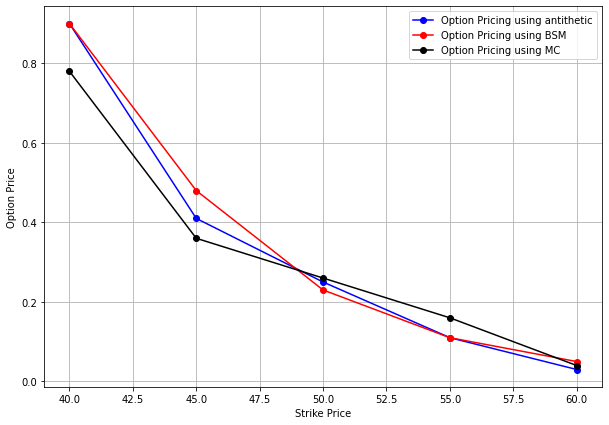
\includegraphics[width=0.8\textwidth]{Option_Pricing_Using_Different_Method}
	\end{center}
	\caption{Option Pricing Using Different Method}
\end{figure}


\noindent Figure 4.1 portrays the movement of option price with respect to strike price for BSM, MC and Antithetic. If we consider BSM as the standard, we can see that the MC and Antithetic is showing good results. In fact, Antithetic is giving better approximation. 

\begin{figure}[H]
	\begin{center}
		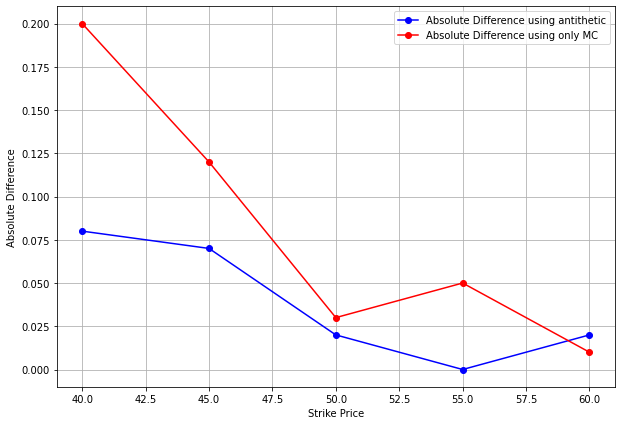
\includegraphics[width=0.8\textwidth]{Absolute_Difference_for_MC_and_Antithetic}
	\end{center}
	\caption{Absolute Difference for MC and Antithetic}
\end{figure}

\noindent From figure 4.2, the absolute difference for Antithetic is lower then MC method.  

\subsection{Barrier Put option: Black Scholes Method vs Monte Carlo Method}

Here, We will create a table for European Call option pricing by Monte Carlo method(with 1000
simulations) using computer generated pseudorandom numbers and then compare those
values with Black-Scholes method results. We are taking stock price, S = 30, strike price, K = From 40 to 60, volatility, vol = 0.3, risk-free rate, r = 0.01, T=1


\begin{table} [H]
\begin{center}
	\begin{NiceTabular}{|c|c|c|c|c|}[hvlines]
		\rowcolor{cyan!20} T & K & BSM & MC & Abs. Diff \\ 
		\Block{5-1}{1}& 40 &   10.59 &   10.77 &   0.18 \\
		& 45 &   15.03 &   15.19 &   0.16 \\
		& 50 &   19.73 &   19.99 &   0.26 \\ 
		& 55 &   24.56 &   24.8 &   0.24 \\
		& 60 &   29.45 &   29.16 &   0.29 \\
	\end{NiceTabular}
\end{center}
\caption{BSM vs MC for Barrier Put}
\end{table}


\noindent Table 4.3 shows that for five different iteration, the difference of BSM and MC is very small. So, MC Method can be told as a good approximation method for evaluating option price of Barrier Put Option.

\begin{figure}[H]
	\begin{center}
		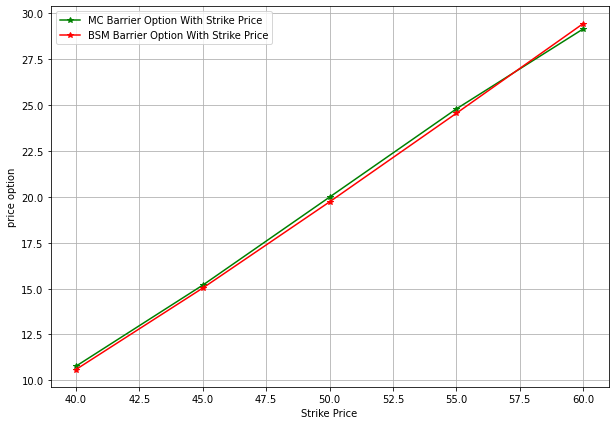
\includegraphics[width=0.8\textwidth]{barrier_mc_bsm}
	\end{center}
	\caption{For Barrier Option MC and BSM With Strike Price}
\end{figure}

\begin{figure}[H]
	\begin{center}
		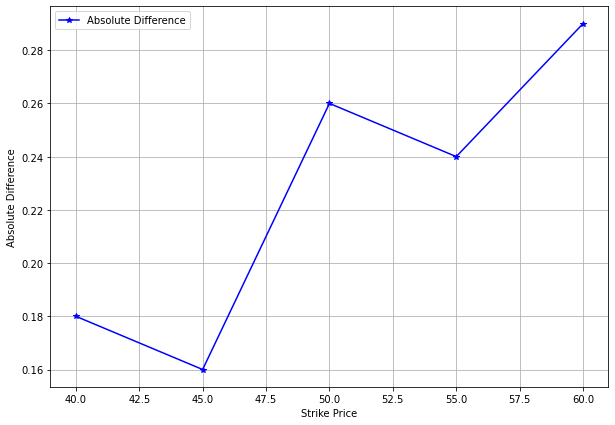
\includegraphics[width=0.8\textwidth]{For_Barrier_Option_Absolute_Difference}
	\end{center}
	\caption{For Barrier Option Absolute Difference}
\end{figure}


\noindent Figure 4.4 shows the absolute difference. As these iterations has been run by some random numbers, values are fluctuating. 